\documentclass{magnolia}

\magtex{tex_driver={pdftex},
        tex_packages={xypic}}
\magfiche{document_nom={Cours Python sur la mémoire},
          auteur_nom={François Fayard},
          auteur_mail={fayard.prof@gmail.com}}
\magcours{cours_matiere={python},
          cours_niveau={mpsi},
          cours_chapitre_numero={5},
          cours_chapitre={Représentation des données}}
\magmisenpage{misenpage_presentation={tikzvelvia},
          misenpage_format={a4},
          misenpage_nbcolonnes={1},
          misenpage_licence={non},
          misenpage_preuve={non},
          misenpage_exemple={oui},
          misenpage_prof={non}}
\maglieudiff{lieu_lycee={Aux Lazaristes},
         lieu_classe={MPSI 1},
         lieu_annee={2019--2020}}
% \magmisenpage{}
% \maglieudiff{}
\magprocess

%\usepackage{minted}
%\usemintedstyle{xcode}

\begin{document}
%BEGIN_BOOK
\hfill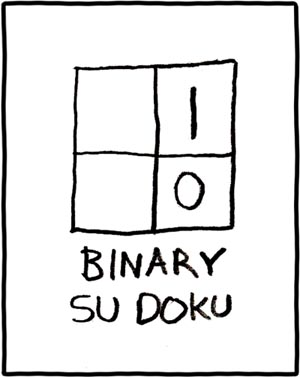
\includegraphics[width=0.25\textwidth]{../../Commun/Images/python-cours-sudoku.jpg}
\magtoc

% quantité mémoire
% integrale

\vspace{2ex}
Un ordinateur possède une mémoire vive, appelée \textsc{Ram} pour \og Random Access
Memory\fg. C'est cette mémoire qui matérialise l'état du système. Concrètement, les
barrettes mémoire contiennent des milliards de condensateurs qui peuvent être
chargés ou déchargés. Lorsqu'un condensateur est chargé, il représente le \emph{bit} 1. S'il est déchargé,
il représente le bit 0.

\begin{center}
\begin{tabular}{|l||c|c|c|c|c|c|c|c|c|c|c|c|}
\hline
condensateur & 0 & 1 & 2 & 3 & 4 & 5 & 6 & 7 & 8 & 9 & 10 & $\ldots$ \\
\hline
état & 0 & 1 & 0 & 0 & 1 & 0 & 1 & 1 & 0 & 0 & 1 & $\ldots$ \\
\hline
\end{tabular}
\end{center}
\noindent
Une succession de 8 bits est appelée un \emph{octet}~: c'est la plus petite quantité
de mémoire adressable par un ordinateur. Les quantités de mémoire se comptent
en kilooctets ($1\ 000\approx 2^{10}$ octets), mégaoctets ($10^6\approx 2^{20}$ octets),
gigaoctets ($10^9\approx 2^{30}$ octets) et téraoctets ($10^{12}\approx 2^{40}$ octets).\\

Dans ce chapitre, nous allons voir comment une succession de 0 et de 1 peut être
utilisée pour représenter des entiers et des nombres flottants.

\section{Les entiers}

\subsection{Décomposition en base $b$}
% \subsection{Décomposition en base $b$}

L'écriture de l'entier 1984 décrit un nombre formé de 4 unités, 8 dizaines, 9 centaines
et 1 millier~:
\[1984 = 4\times 10^0 +\ 8\times 10^1 + \ 9 \times 10^2 + \ 1\times 10^3.\]
Le choix de faire des paquets en utilisant des puissances de 10 est cependant arbitraire.
On peut tout aussi bien décider d'utiliser des puissances de 2, 12, 16 ou 60. Si l'on choisit
d'utiliser des puissances de $b$, on dit qu'on décompose notre nombre en base $b$.

\begin{proposition}
Soit $b\geq 2$ un entier et $w\in\N$. Alors, pour tout $n\in\interefo{0}{b^w}$, il existe un unique $w$-uplet $(d_0,d_1,\ldots,d_{w-1})$ d'éléments de $\interefo{0}{b}$ tel que
\[n=\sum_{k=0}^{w-1} d_k b^k.\]
\end{proposition}

\begin{preuve}
Nous allons prouver ce résultat par récurrence sur $n$. Soit $b\geq 2$ un entier. Pour tout $n\in\N$, on pose
\begin{center}
$\mathcal{H}_n\defeq$ \og
\begin{minipage}[t]{0.6\linewidth}
Quel que soit $m\in\interefo{0}{b^n}$, il existe un unique $n$-uplet $(d_0,d_1,\ldots,d_{n-1})$ d'éléments de $\interefo{0}{b}$ tel que
$m=\sum_{k=0}^{n-1} d_k b^k$.\fg
\end{minipage}
\end{center}
\begin{itemize}
\item \emph{$\mathcal{H}_0$ est vraie}~: En effet, si $m\in\interefo{0}{1}$, alors $m=0$. Puisque qu'il existe un unique $0$-uplet d'éléments de $\interefo{0}{1}$ et qu'une somme vide est égale à 0, $\mathcal{H}_0$ est prouvée.
\item $\mathcal{H}_n\implique\mathcal{H}_{n+1}$~: Soit $n\in\N$. On suppose que $\mathcal{H}_n$ est vraie. Montrons que $\mathcal{H}_{n+1}$ est vraie. Soit $m\in\interefo{0}{b^{n+1}}$ et montrons qu'il existe un unique $(n+1)$-uplet $(d_0,\ldots,d_n)$ d'éléments de $\interefo{0}{b}$ tel que
\[m=\sum_{k=0}^{n} d_k b^k.\]
\begin{itemize}
\item \emph{Existence~:} On effectue la division euclidienne de $m$ par $b$. Il existe donc $q\in\N$ et $d_0\in\interefo{0}{b}$ tels que $m=qb+d_0$. Puisque $qb+d_0< b^{n+1}$, on en déduit que $qb<b^{n+1}$, puis que $q<b^n$. Puisque $\mathcal{H}_n$ est vraie, il existe donc un $n$-uplet $(d_1,\ldots,d_n)$ d'éléments de $\interefo{0}{b}$ tels que $q=\sum_{k=0}^{n-1} d_{k+1} b^k$. Alors
\begin{eqnarray*}
m & = & d_0+\p{\sum_{k=0}^{n-1} d_{k+1} b^k}b = d_0+\sum_{k=0}^{n-1} d_{k+1} b^{k+1}\\
  & = & d_0+\sum_{k=1}^{n} d_{k} b^{k} = \sum_{k=0}^{n} d_{k} b^{k}.
\end{eqnarray*}
\item \emph{Unicité~:} Soit $(d_0,\ldots,d_n)$ et $(e_0,\ldots,e_n)$ deux $(n+1)$-uplets d'éléments de $\interefo{0}{b}$ tels que
\[m=\sum_{k=0}^n d_k b^k \quad\et\quad m=\sum_{k=0}^n e_k b^k.\]
Montrons que pour tout $k\in\intere{0}{n}$, $d_k=e_k$. On a
\[m=\sum_{k=0}^{n} d_{k} b^{k} = \underbrace{\p{\sum_{k=1}^n d_k b^{k-1}}}_{\in\Z}b + \underbrace{d_0}_{\in\interefo{0}{b}}\]
donc $d_0$ est le reste de la division euclidienne de $m$ par $b$. De même, $e_0$ est le reste de la division euclidienne de $m$ par $b$. Par unicité du reste de la division euclidienne, on en déduit que $d_0=e_0$. De même, par unicité du quotient de la division euclidienne, on en déduit que
\[\sum_{k=1}^n d_k b^{k-1}=\sum_{k=1}^n e_k b^{k-1},\]
ce qui donne, après réindexation
\[\sum_{k=0}^{n-1} d_{k+1} b^k=\sum_{k=0}^{n-1} e_{k+1} b^k.\]
On pose alors $m'\defeq \sum_{k=0}^{n-1} d_{k+1} b^k$. Puisque $0\leq d_{k+1}\leq b-1$ pour tout $k\in\intere{0}{n-1}$, on en déduit que
\[0\leq m' \leq \sum_{k=0}^{n-1} (b-1)b^k=(b-1)\sum_{k=0}^{n-1} b^k=(b-1)\frac{1-b^n}{1-b}=b^n-1.\]
Puisque $\mathcal{H}_n$ est vraie, on en déduit que pour tout $k\in\intere{1}{n}$, $d_k=e_k$, ce qui finit de prouver l'unicité.
\end{itemize}
On a donc prouvé que $\mathcal{H}_{n+1}$ est vraie.
\end{itemize}
Par récurrence sur $n$, on en déduit que $\mathcal{H}_n$ est vraie pour tout $n\in\N$.
\end{preuve}

\begin{remarques}
\remarque On parle de \emph{décomposition en base $b$} de l'entier $n$. Les $d_k$ sont appelés
  \emph{chiffres} de $n$ en base $b$.
\remarque Les chiffres correspondant aux plus grandes puissances de $b$ sont dits
    \emph{plus significatifs} ou de \emph{poids fort}. Ceux qui correspondent aux
    petites puissances de $b$ sont dits \emph{moins significatifs} ou de
    \emph{poids faible}.
\remarque Pour tout $n\in\Ns$, il existe un unique $w\in\Ns$ et un unique
  $w$-uplet $(d_0,d_1,\ldots,d_{w-1})$ d'éléments de $\interefo{0}{b}$ tel que
  $d_{w-1}\neq 0$ et $n=\sum_{k=0}^{w-1} d_k b^k$. On écrit
  \[n=\underline{d_{w-1}\cdots d_1 d_0}_{b}.\]
  Lorsqu'on parle de \emph{la} décomposition de $n$ en base $b$, c'est de cette écriture
  qu'il s'agit. 
  Par exemple $13=\underline{13}_{10}$ car $13=3\times 10^0 + 1\times 10^1$ et
  $13=\underline{1101}_{2}$ car $13=1\times 2^0+0\times 2^1+1\times 2^2+1\times 2^3$. Par convention, la décomposition de 0 est vide, quelle que soit la base.
\remarque En base 2, les valeurs possibles pour un chiffre sont $0$ et $1$; on
  parlera indifféremment de \emph{bit} ou de chiffre. Étant donné l'importance de la
  base 2 en informatique, il est bon de connaitre les premières puissances de 2.
  \[\begin{array}{|c|c|c|c|c|c|c|c|c|c|c|}
  \hline
  \raisebox{10pt}{} 2^0 & 2^1 & 2^2 & 2^3 & 2^4 & 2^5 & 2^6 & 2^7 & 2^8 & 2^9 & 2^{10} \\
  \hline
  \raisebox{10pt}{} 1 & 2 & 4 & 8 & 16 & 32 & 64 & 128 & 256 & 512 & 1\ 024 \\
  \hline
  \end{array}\]
\remarque Si la base est supérieure à dix, on a un problème pour l'écriture~: il y a moins
  de chiffres usuels que de chiffres de la base. Le seul cas que l'on rencontre en pratique
  est celui de la base 16 dite \emph{hexadécimale}. La convention est d'utiliser les lettres
  de \verb!A! à \verb!F! pour représenter les chiffres de 10 à 15. 
\remarque Les bases 2, 16 et dans une moindre mesure 8, sont couramment utilisées
  en informatique. Par conséquent, il est possible d'écrire les littéraux directement dans
  ces bases. En Python, la syntaxe est~:
\begin{pythoncode}
In [1]: 0b10010
Out[1]: 18

In [2]: 0xff
Out[2]: 255

In [3]: 0o77
Out[3]: 63
\end{pythoncode}
\remarque Si l'on veut obtenir les chiffres de 137 en base 10, on commence par écrire
  que $137 = 13 \times 10 + 7$~: on effectue la division euclidienne de 137 par 10.
  Le chiffre de poids faible $d_0$ est donc $7$, et avant cela on a les chiffres de 13. 
  De même, $13 = 1 \times 10 + 3$, donc $d_1 = 3$, et on continue en remplaçant $13$ par 1. Enfin
  $1 = 0 \times 10 + 1$, donc $d_2 = 1$. On remplace $1$ par $0$ et on a terminé car $0$
  n'a «~pas de chiffre~». On a donc $137 = \underline{137}_{10}$.
\remarque Si au contraire on dispose de la liste des chiffres en base $b$ et que l'on
  souhaite obtenir $n$, le plus efficace est de remarquer  que
  \[\sum_{k = 0}^{w-1} d_k b^k
  = d_0 + b\p{d_1 + b\p{d_2 + \cdots b \p{d_{w-2} + b d_{w-1}}}}.\]
  Cette écriture est à la base de l'algorithme de Horner~: on part de 0 et on
  multiplie successivement notre valeur par 10 avant de lui ajouter $d_k$, pour toutes
  les valeurs de $k$ allant en décroissant de $w-1$ à $0$. Si l'on souhaite
  calculer $\underline{137}_{10}$, on effectue donc les calculs
  \[
    0 \xrightarrow[\times 10+1]{}  1
    \xrightarrow[\times 10+3]{}  13
    \xrightarrow[\times 10+7]{} 137.
  \]
\end{remarques}

\begin{exos}
  \exo Calculer $\underline{1000110}_2$ et $\underline{C7}_{16}$.
  \exo Donner l'écriture binaire de 59 et de 31. Quel phénomène général peut-on
    remarquer dans le deuxième cas ?
  \exo Comment s'écrit $\underline{102}_3$ en base 5 ?
\end{exos}
\vspace{2ex}
La fonction \verb!eval_lsd(b: int, d: list[int]) -> int! (\verb!lsd! pour
  least significant digit)
  renvoie l'entier dont l'écriture en base $b$ est \[\underline{d_{w - 1}\dots d_{0}}_{b}\]
  en utilisant l'algorithme de Horner.
\begin{pythoncodeline}
def eval_lsd(b, d):
    """eval_lsd(b: int, d: list[int]) -> int"""
    w = len(d)
    n = 0
    for k in range(w):
        n = n * b + d[w - 1 - k]
    return n
\end{pythoncodeline}

La fonction \verb!digits_lsd(b: int, n: int) -> list[int]!
  renvoie la liste des chiffres de $n$ en base $b$, le chiffre le moins significatif étant en premier.
\begin{pythoncodeline}
def digits_lsd(b, n):
    """digits_lsd(b: int, n: int) -> list[int]"""
    d = []
    while n > 0:
        d.append(n % b)
        n = n // b
    return d
\end{pythoncodeline}
Ces deux fonctions sont bien entendu à connaitre sur le bout des doigts.\\


\begin{proposition}
  Soit $b \geq 2$ un entier. Un entier $n > 0$ s'écrit avec $w=1 + \lfloor \log_b (n) \rfloor$ chiffres
    en base $b$.
  \end{proposition}

\vspace{2ex}
Les opérations d'addition et de multiplication apprises à l'école primaire fonctionnent
tout aussi bien en base $b\geq 2$ qu'en base 10. Entrainez-vous avec les exercices suivants pour
vous convaincre de cela.
\vspace{2ex}
\begin{exos}
\exo Effectuer l'addition $\underline{100110}_2 + \underline{1011}_2$
  en base 2, c'est-à-dire sans jamais convertir un nombre en base 10.
\exo Effectuer la multiplication $\underline{100110}_2 \times \underline{1011}_2$
  en base 2.
\exo Écrire les tables de multiplication en base 3. Calculer
  le produit $\underline{1022}_3 \times \underline{221}_3$ en travaillant en base 3.
\end{exos}
\vspace{2ex}
La décomposition en base 2 nous permet de revenir sur l'algorithme d'exponentiation
rapide dont nous avons donné une version récursive dans le chapitre sur les fonctions et
dont nous donnons ici une version itérative. Étant donné $n\in\N$, on effectue
sa décomposition en base 2
\[n=\sum_{k=0}^{w-1} d_k 2^k\]
et on remarque que pour tout $x$
\[x^n=x^{\sum_{k=0}^{w-1} d_k 2^k}=\prod_{k=0}^{w-1} \cro{x^{\p{2^k}}}^{d_k}.\]
Comme $d_k\in\ens{0,1}$, quel que soit $k\in\intere{0}{w-1}$, le terme entre crochets
est soit présent dans le produit (si $d_k=1$) soit absent (si $d_k=0$). De plus, il est aisé de calculer les
valeurs successives de $x^{2^k}$ car chaque terme est le carré du précédent.
On obtient ainsi l'algorithme d'exponentation rapide dans sa version itérative.

\begin{pythoncodeline}
def expo(x, n):
    """expo(x: int, n: int) -> int"""
    ans = 1
    y = x
    m = n
    while m > 0:
        if m % 2 == 1:
            ans = ans * y
        y = y * y
        m = m // 2
    return ans
\end{pythoncodeline}

\subsection{Représentation mémoire des entiers non signés}

La décomposition en base 2 nous donne un moyen de représenter les nombres positifs
à l'aide d'une séquence de bits.  Comme cette décomposition s'effectue uniquement pour
les entiers positifs, on parle de représentation des entiers \emph{non signés}. C'est cette
représentation que les processeurs utilisent pour manipuler les entiers non signés. Il ne sont
cependant capables que de travailler avec des entiers ayant une largeur $w$ fixée.
Aujourd'hui, un processeur 64~bits peut travailler avec des entiers codés sur 8, 16, 32
ou 64 bits.

\begin{proposition}
Pour une largeur de $w\in\N$, le plus grand entier non signé représentable est $2^{w} - 1$.
\end{proposition}

Avec 8 bits, on peut coder tous les entiers entre 0 et $2^8-1=255$. 
Avec 16 bits, on peut coder tous les entiers entre 0 et $2^{16}-1=65\ 535$.
Avec 32 bits on peut coder
tous les entiers entre 0 et $2^{32}-1=4\,294\,967\,295$, soit quelques milliards. Avec
64 bits on peut coder tous les entiers entre 0 et quelques milliards de milliards, ce qui
est suffisant pour de nombreuses applications.\\

Ces représentations sur une largeur fixe ont cependant un défaut~: la somme et le produit de deux
entiers représentables ne sont pas toujours représentables. Par exemple, avec une largeur
de 8 bits, 250 et 12 sont représentables, mais $250+12$ ne l'est pas. Lorsque ce problème
survient, on dit qu'il y a un \emph{dépassement de capacité} (\emph{overflow} en anglais)
et le résultat obtenu est calculé modulo 256. Dans notre exemple, le calcul sur 8 bits
de $250+12$ donnera donc 6~! Certains langages comme le C ne cachent pas cette
caractéristique des processeurs et le programmeur a la responsabilité de s'assurer que
ce problème n'arrive jamais (ou d'agir en conséquence).
Python travaille quant à lui avec des entiers de taille variable. L'avantage est qu'il peut manipuler des
entiers aussi grands que l'on souhaite; on ne risque pas de dépassement de capacité.
L'inconvénient est que les opérations usuelles sur ces entiers sont bien plus lentes
qu'en C et que leur temps d'exécution dépend de la taille des
entiers.




\subsection{Représentation mémoire des entiers signés}


Les entiers considérés pour le moment étaient supposés positifs,
mais les processeurs proposent bien évidemment de travailler avec des types
\emph{signés}, qui permettent de représenter des valeurs négatives.
D'une manière ou d'une autre, il est clair que le signe nous \og coutera \fg un bit : il faut
stocker l'information $+$ ou  $-$. Il est assez naturel d'imaginer la stratégie
suivante :
\begin{itemize}
  \item Le bit le plus significatif détermine le signe : un 1 signifie que le nombre est
  positif, un 0 qu'il est négatif.
  \item La valeur absolue du nombre est stockée de manière standard sur les autres bits.
\end{itemize}
Implicitement, nous considérons ici que l'on travaille avec
des entiers d'une largeur $w$ fixée. Ainsi, l'expression \emph{bit le plus
  significatif} désigne le bit $d_{w-1}$ de poids maximal dans cette largeur, ce qui explique pourquoi il peut être égal à zéro.\\


Bien que cette méthode paraisse raisonnable, elle a deux défauts~:
\begin{itemize}
  \item Le nombre 0 a deux représentations : $00\dots0$ et $10\dots0$. Cela a pour
  conséquence de ne pouvoir stocker que $2^w - 1$ valeurs différentes, par exemple les entiers
  de $-(2^{w-1} - 1)$ à $2^{w- 1} - 1$ inclus. On perd une place puisque zéro en prend deux.
  \item Les opérations arithmétiques usuelles ne sont pas très simples à effectuer~: essentiellement,
  pour ajouter deux nombres, on est obligé de regarder leur bit de poids fort pour déterminer
  leur signe et de distinguer les cas.
\end{itemize}

En réalité, aucun ordinateur n'utilise cette représentation pour les entiers signés.
L'immense majorité utilise la représentation par \emph{complément à deux}.

\begin{proposition}
Soit $w\in\Ns$. Pour tout $n\in\interefo{-2^{w-1}}{2^{w-1}}$, il existe un unique $w$-uplet
$(b_0,b_1,\ldots,b_{w-1})$ de bits tel que
\[n=\p{\sum_{k=0}^{w-2} b_k 2^k} - b_{w-1}2^{w-1}.\]
\end{proposition}

\begin{remarques}
\remarque Le bit $b_{w-1}$ est nul si et seulement si $n\geq 0$. Si tel est le cas
  $(b_0,\ldots,b_{w-1})$ est la décomposition de $n$ en base 2.
  Sinon $n<0$, $b_{w-1}=1$ et $(b_0,\ldots,b_{w-1})$ est la décomposition de
  $n + 2^w$ en base 2.
\remarque On appelle valeur en \emph{complément à deux} de la suite
de bits $(b_0, \ldots, b_{w-1})$ l'entier
\[\p{\sum_{k=0}^{w-2} b_k 2^k} - b_{w-1}2^{w-1}.\]
  On dit que le bit de poids fort a un poids négatif.
\remarque Une même suite de bits $(b_0, \ldots, b_{w-1})$ dans une 
  largeur $w$, correspondra donc à deux entiers différents :
  $\sum_{k = 0}^{w - 1}b_{k} 2^{k}$ en non signé et
  $\sum_{k = 0}^{w - 2}b_{k}2^{k} -b_{w - 1}2^{w - 1}$ en signé par
  complément à deux.
  Fixons par exemple
  $w \defeq 4$, et notons respectivement ${\rm v}_{4}(b_{3}b_{2}b_1 b_0)$ et ${\rm vs}_{4}(b_3 b_2 b_1 b_0)$, les
  valeurs non signées et signées associées à une suite de bits.
  \begin{itemize}
    \item $\ {\rm vs}_{4}(0000) = {\rm v}_{4}(0000) = 0.$
    \item $\ {\rm vs}_{4}(0100) = {\rm v}_{4}(0100) = 4.$
    \item $\ {\rm vs}_{4}(1100) = -8 + 4 = -4$ et ${\rm v}_{4}(1100) = 8 + 4 = 12.$
    \item $\ {\rm vs}_{4}(1111) = -8 + 4 + 2 + 1 = -1$ et ${\rm v}_{4}(1111) = 8 + 4 + 2 + 1 = 15.$
  \end{itemize}
\end{remarques}

\begin{exoUnique}
  \exo
  On fixe $w \defeq 8$.
  \begin{questions}
    \item Quel est le plus grand entier non signé représentable, c'est-à-dire
          la plus grande valeur ${\rm v}_{8}(bits)$ que l'on peut obtenir ?
    \item Quels sont les plus petits et plus grands entiers signés
          représentables ?
    \item Quelle suite de bits donne ${\rm vs}_{8}(bits) = 0$ ? $127$ ?
          $-1$ ? $-128$ ?
  \end{questions}
% \exo \emph{Complément à deux et complément à un}~: 
%   Si $n \in \llbracket 0, 2^w - 1 \rrbracket$ est un entier codé en binaire sur
%   $w$ bits, son \emph{complément à un} est l'entier obtenu en inversant tous
%   les bits de $n$ (les 1 deviennent des 0 et inversement). Justifier que le
%   complément à deux de $n$ peut être obtenu en ajoutant un au complément à
%   un de $n$.
\end{exoUnique}

\begin{proposition}
  Pour une largeur $w\in\Ns$
  \begin{itemize}
    \item Le plus grand entier signé représentable en complément à 2 est
          $2^{w - 1} - 1$.
    \item Le plus petit entier signé représentable en complément à 2 est
          $-2^{w - 1}$.
  \end{itemize}
\end{proposition}

\begin{remarques}
  \remarque \emph{Explosion d'Ariane 5} :
  Le vol inaugural de la fusée Ariane 5 a eu lieu le 4 juin 1996.
  Comme le montre l'illustration ci-dessous, il s'est terminé, un peu
  moins de 37 secondes après le décollage, par ce que nous appellerons
  pudiquement un \textsc{Rud} (\emph{Rapid Unplanned Dissassembly}).
  \begin{center}
    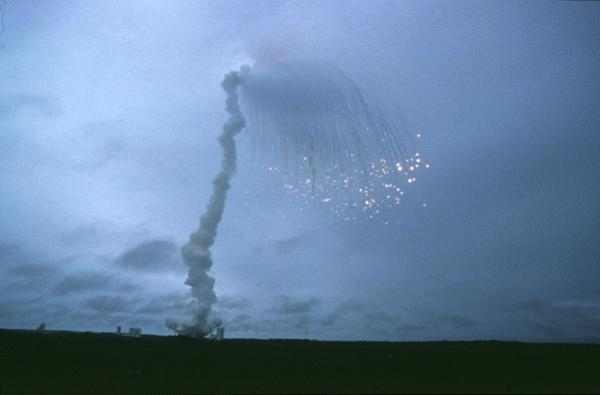
\includegraphics[width = 12cm]{../../Commun/Images/info-cours-memoire-explosion_ariane}\\
    Dommage.
  \end{center}
  \vspace{1ex}
  La fusée et son chargement avaient couté 500
  millions de dollars. La commission d'enquête a rendu son rapport au bout de
  deux semaines. Il s'agissait d'une erreur de programmation dans le système
  inertiel de référence. À un moment donné, un nombre codé en virgule flottante
  qui représentait la vitesse horizontale de la fusée par rapport à la
  plateforme de tir était converti en un entier signé sur 16 bits. Malheureusement, le
  nombre en question était plus grand que 32\ 767 et la conversion a été incorrecte.
  \vspace{1ex}
  \begin{center}
    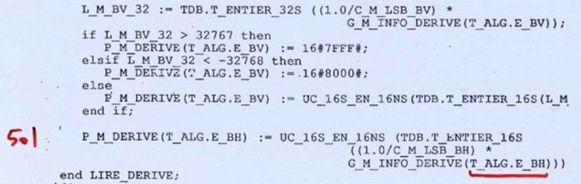
\includegraphics[width = 14cm]{../../Commun/Images/info-cours-memoire-code_ariane}\\
    Extrait du code source (en \textsc{Ada}) d'Ariane 5. On peut voir
      un certain nombre\\ de conversions d'un entier 32 bits
      vers un entier 16 bits
      avec protection contre les dépassements\\ de
      capacité, et, soulignée en rouge, une conversion  non protégée d'un\\ flottant vers
      un entier 16 bits.
  \end{center}
  \remarque
    L'année 2012 a été marquée par une contribution majeure au patrimoine
    culturel de l'humanité : la vidéo \emph{Gangnam Style}. À cette
    époque, le nombre de vues d'une vidéo YouTube était codé 
    sur un entier 32 bits signé.
    Bien évidemment, ce choix, qui limite le nombre de vues à
    \nombre{2\ 147\ 483\ 647}, n'était absolument pas adapté à un
    chef-d'œuvre de cette ampleur. Début 2014, il est devenu évident
    qu'on allait bientôt avoir un dépassement de capacité. Fort heureusement,
    YouTube a apporté la modification nécessaire à temps : les vues sont
    maintenant codées sur un entier signé de 64 bits, ce qui laisse de la marge, la valeur maximale étant
    \nombre{9\ 223\ 372\ 036\ 854\ 775\ 807}. \emph{Baby shark} peut rester
    tranquille pour de nombreuses années.
  \end{remarques}

\begin{proposition}
  Pour toute largeur $w\in\N$ et toute suite de bits $(b_0, \ldots, b_{w-1})$, on a
  \begin{displaymath}
    {\rm v}_{w}(bits) \equiv {\rm vs}_{w}(bits) \mod{2^{w}}.
  \end{displaymath}
\end{proposition}

\begin{remarques}
  \remarque
  Cette propriété est la raison d'être de la représentation par complément
  à deux.
  \remarque
  Nous n'allons pas rentrer dans les détails qui ne nous intéressent pas
  vraiment, mais l'avantage principal de la représentation en complément à
  deux, illustré par l'exercice ci-dessous, est qu'on peut utiliser
  essentiellement le même circuit physique pour les opérations arithmétiques
  sur les entiers signés et non signés.
\end{remarques}
\vspace{2ex}
\begin{exoUnique}
  \exo
  \begin{questions}
    \item Poser les additions binaires suivantes :
          \begin{multicols}{4}
            \begin{tabular}{rl}
              & 1011 \\
              + & 0111 \\
              \hline
              &
            \end{tabular}
            \begin{tabular}{rl}
              & 1001 \\
              + & 0011 \\
              \hline
              &
            \end{tabular}
            \begin{tabular}{rl}
              & 1001 \\
              + & 1011 \\
              \hline
              &
            \end{tabular}
            \begin{tabular}{rl}
              & 0101 \\
              + & 0011 \\
              \hline
              &
            \end{tabular}
          \end{multicols}
    \item Interpréter ces additions comme des opérations sur des
          entiers non signés de 4 bits. On ne gardera donc que les
          quatre bits les moins significatifs du résultat.
          Mathématiquement, cela revient à faire quoi ?
    \item Reprendre la question précédente en faisant cette fois
          une interprétation signée, en complément à deux, sur
          quatre bits.
    \item Quel critère simple, portant sur les deux bits de retenue
          de poids les plus forts, peut-on utiliser pour déterminer
          s'il y a eu un «~vrai~» dépassement de capacité ?
          Par \og vrai \fg dépassement de capacité, on entend une
          situation dans laquelle le résultat mathématique de
          l'opération n'est pas représentable avec la largeur fixée.
  \end{questions}
\end{exoUnique}
\vspace{2ex}


% Si on veut à la fois stocker des entiers positifs et négatifs, une astuce est nécessaire. Si on représente les nombres sur $n$ bits, on va choisir de représenter tous les entiers entre et $-2^{n-1}$ et $2^{n-1}-1$ inclus. On parle de représentation des entiers \emph{signés}.
% \begin{itemize}
% \item Tous les nombres entre $0$ et $2^{n-1}-1$ sont représentés par leur décomposition binaire.
% \item Pour les nombres $m$ entre $-2^{n-1}$ et $-1$, on les représente par la décomposition binaire de $m+2^n$. Autrement dit, on les stocke modulo $2^n$.  
% \end{itemize}
% Cette manière de stocker les nombres est très pratique pour les ordinateurs. On l'appelle méthode du \emph{complément à 2}. Par exemple, si $n=8$, $-1$ est représenté par $\underline{11111111}_2$.

% \begin{exoUnique}
% \exo Donner la représentation de $67$, de $-31$ et de $0$ en complément à 2 sur 8 bits.
% 	\`A l'inverse, déterminer l'entier codé par $\underline{10011011}_2$.
% \end{exoUnique}
% \begin{sol}
% $67 $ est toujours représenté par \begin{tabular}{|c|c|c|c|c|c|c|c|}\hline 0 & 1 & 0 & 0 & 0 & 0 & 1 & 1\\ \hline \end{tabular}.

% $-31+256 = 225 = 2\times112 +1 = 2^2\times 56 +1 = 2^3\times 28 +1 = 2^4\times 14+1=2^4\times(8+4+2)+1 = 2^7+2^6+2^5+2^0$ donc $-31$ est représenté par \begin{tabular}{|c|c|c|c|c|c|c|c|}\hline 1 & 1 & 1 & 0 & 0 & 0 & 0 & 1\\ \hline \end{tabular}.

% $0$ a une seule représentation : 
% \begin{tabular}{|c|c|c|c|c|c|c|c|}\hline 0 & 0 & 0 & 0 & 0 & 0 & 0 & 0\\ \hline \end{tabular}.

% Le code \underline{10011011} représente un entier $x<0$. Ainsi, $x+2^8=2^7+2^4+2^3+2^1+2^0=155$. D'où $x=155-256=-101$.

% \end{sol}

% Dans de nombreux langages de programmation de bas niveau comme le C, seuls les nombres stockés sur $n$ bits (avec $n=8,16,32$ ou 64) sont disponibles et les opérations d'addition et de multiplication sont toutes écrites modulo $2^n$. Par exemple, si on travaille en 8 bits et que l'on ajoute 1 à 127, on tombe sur $-128$! En OCaml, pour des raisons d'optimisation, les entiers sont des entiers signés sur 63~bits. L'avantage de ce stockage en mémoire pour les nombres négatifs est que le processeur peut ajouter ou multiplier les nombres de la même manière sans se soucier de leur signe.\\

% Enfin, certains ordinateurs stockent les bits de poids faible en premier (Little Indian) alors que d'autres stockent les bits de poids fort en premier (Big Indian). Ces dénominations proviennent des \og Voyages de Gulliver\fg de \textsc{Jonathan Swift} où certains indiens ouvrent les oeufs du côté le plus pointu tandis que d'autres les ouvrent du côté le plus rond. La plupart des ordinateurs actuels utilisent le format Little Indian et on a moins de pagaille lorsque les ordinateurs s'échangent des données.\\

% % \begin{exercicepython}{}
% % On suppose que l'on utilise une machine représentant les entiers signés sur $8$ bits. 
% % \begin{questions}
% % \question Quels sont les entiers représentables~? 
% % \question Comment s'écrivent $-7$, $7$,$13$,$-1$, $3$?
% % \end{questions}
% % \end{exercicepython}

% En Python, le type \verb_int_ permet de représenter les entiers sans limite de taille. En interne, le langage adapte automatiquement la représentation en fonction de la taille de l'entier. Pour faire simple, on peut dire que Python stocke le signe de l'entier sur 1~bit. Il stocke ensuite sa valeur absolue en tant qu'entier non signé en utilisant 64~bits si il est inférieur à $2^{64}-1$, 128 bits si il est inférieur à $2^{128}-1$, etc. La représentation exacte est légèrement différente, mais l'idée est là.

% \begin{remarques}
% \remarque La démonstration de la proposition précédente nous donne l'algorithme de la décomposition de $m$ en base $b$. On pose $u_0\defeq m$. Alors $d_0$ est le reste de la division euclidienne de $u_0$ par $b$. On note alors $u_1$ le quotient de la division euclidienne de $u_0$ par $b$. Alors $d_1$ est le reste de la division euclidienne de $u_1$ par $b$. On note alors $u_2$ le quotient de la division euclidienne de $u_1$ par $b$. On continue ce processus jusqu'à ce que $u_n=0$.


	


% \remarque Lorsqu'on décompose un nombre en base 16, on utilise $A$ pour représenter 10, $B$ pour représenter 11, jusqu'à $F$ pour représenter 15. Par exemple, puisque $179=3\times 16^0+11\times 16^1$, on écrit $179=\underline{B3}_{16}$.
% \remarque Pour $b=2$, la proposition précédente nous dit simplement que l'application de $\ens{0,1}^n$ dans $\intere{0}{2^n-1}$ qui à $(d_0,\ldots,d_{n-1})$ associe
%   \[\sum_{k=0}^{n-1} d_k 2^k\]
%   est une bijection.
% \end{remarques}



% \begin{exos}
% \exo a
% \end{exos}


% Nous utilisons tous la notation décimale qui est une décomposition en base 10. En effet, le nombre 85 s'écrit
% \[85=5\times 10^0+8\times 10^1\]
% mais on peut aussi décomposer ce nombre en base 2
% \[85=1\times 2^0 + 0\times 2^1 + 1\times 2^2 + 0\times 2^3 + 1\times 2^4 + 0\times 2^5 + 1\times 2^6\]
% en base 8, ou en base 16~:
% \[85=5\times 8^0 + 2\times 8 + 1\times 8^2 \et
%   85=5\times 16^0 + 5 \times 16^1\]
% En mettant les \og chiffres de poids fort\fg en tête, on écrit donc
% \[85=\underline{85}_{10}, \quad 85=\underline{1010101}_{2} \quad 85=\underline{125}_8\]
% Enfin, pour la base 16 (hexadécimale), on utilise $A$ pour représenter 10, $B$ pour représenter 11, jusqu'à $F$ pour représenter 15. Par exemple, $85=\underline{55}_{16}$ et $31=\underline{1F}_{16}$.

% \begin{exos}
% \exo Décomposer 45 en base 10, en base 5, en base 2.
% \exo Donner l'écriture en base 16 de $85$, puis celle de $31$.
% \end{exos}



% \subsection{Algorithmes de décomposition et de reconstruction}


\section{Les nombres flottants}



\subsection{Représentation mémoire des flottants}

Pour écrire un nombre réel de manière approchée, les physiciens ont pris l'habitude
d'utiliser l'écriture scientifique. Par exemple
\[\e^{\pi}\approx 23.14 = 2.314 \times 10^1 =\p{2+\frac{3}{10}+\frac{1}{10^2}+\frac{4}{10^3}}\times 10^1.\]
On dit qu'un tel nombre est représenté avec 4 chiffres significatifs. Remarquons que
contrairement aux entiers naturels, qui admettent tous une décomposition en base $b$,
seuls les nombres décimaux peuvent s'écrire de manière exacte sous la forme
\[\pm\p{\sum_{k=0}^{p-1} \frac{m_k}{10^k}}\times 10^e\]
où $m_k\in\intere{0}{9}$. Même certains nombres rationnels comme $1/3$ ne peuvent
pas s'écrire de la sorte. Bien entendu, ces remarques faites en base 10 sont aussi
valables en base 2, plus familière des ordinateurs.

% nous avons l'habitude d'utiliser l'écriture décimale de $x$ et de la tronquer (ou de faire un arrondi). Par exemple,
% une valeur approchée de $\pi$ est  $3,14$ à $10^{-2}$ près. Ainsi 
% \[\pi \approx 3.14 = 3 + \dfrac{1}{10}+\dfrac{4}{10^2}.\]
% On peut ainsi montrer que tout nombre réel $x$ non nul est limite lorsque $n$ tend vers $+\infty$ de
% la suite de terme général
% \[s\p{\sum_{k=0}^{n} \frac{m_k}{10^k}} 10^e\]
% où $s\in\ens{-1,1}$, $(m_n)$ est une suite d'entiers de $\intere{0}{9}$, $m_0\neq 0$ et $e\in\Z$. Pour les nombres décimaux, $m_k$ est nul à partir d'un certain rang. Par
% exemple
% \[12789 = 1.2789 \times 10^{4}, \qquad -423 = -4.23\times 10^2, \qquad  0.0064001 =  6.4001\times 10^{-3}.\]


% \begin{proposition}
% Soit $b$ un entier tel que $b\geq 2$ et $x$ un réel non nul. Alors il existe un unique triplet $(s,m,e)$ où $s\in\ens{+1,-1}$, $(m_k)$ est une suite d'éléments de $\intere{0}{b-1}$ qui n'est pas égale à $b-1$ à partir d'un certain rang et $e\in\Z$ tels que
% \[x = s\p{\sum_{k=0}^{+\infty} \frac{m_k}{b^k}} b^e\]
% On dit que cette décomposition est l'écriture scientifique de $x$ en base $b$.
% \end{proposition}

% Le somme infinie fait référence à limite de la suite de terme général
% \[u_n\defeq\sum_{k=0}^n \frac{m_k}{b^k}\]
% qui est bien convergente comme suite croissante, majorée par $b$. Pour $b=10$, on obtient l'écriture classique sous forme scientifique. Par exemple

% Il est à noter qu'il convient bien d'imposer à la suite de ne pas être égale à $b-1$ à partir d'un certain rang pour avoir l'unicité. En effet
% \[1=1.000\cdots\times 10^0 \et 1=9.999\cdots\times 10^{-1}.\]
% On dit qu'un nombre est décimal lorsque pour $b=10$, la suite $(m_k)$ est nulle à partir d'un certain rang. Remarquons que pour les nombres rationnels, la suite $(m_k)$ est périodique à partir d'un certain rang. Par exemple~:
% \[\frac{22}{7}=3.142857\underline{142857}\cdots\times 10^0\]
% On peut même montrer que cette propriété caractérise les nombres rationnels.
% Pour calculer effectivement les $m_k$ pour un nombre strictement positif $x$, on commence par déterminer $e$ tel que $y=x/b^e\in\interfo{1}{b}$.

% \begin{exercicepython}{}
% Donner une mani\`ere de calculer $m_k$ \`a partir de $y$ et $b$.
% \end{exercicepython}

% \begin{exercicepython}{}
% Donner le développement décimal de $0.1$ et $0.3$ en base 10, puis en base 2.
% \end{exercicepython}


\begin{definition}
Soit $p\in\Ns$. On dit qu'un réel $x$ est un nombre flottant représentable avec une mantisse de $p$ bits lorsqu'il existe $m_0,\ldots,m_{p-1}\in\ens{0,1}$ et $e\in\Z$ tels que
\[x=\pm\p{\sum_{k=0}^{p-1} \frac{m_k}{2^k}}2^e.\]
Si $x$ est non nul, il est possible d'imposer $m_0=1$; cette écriture est alors unique. L'ensemble des nombres flottants représentables avec une mantisse de $p$ bits est noté $\mathcal{F}_p$.  
\end{definition}

\begin{remarques}
\remarque 
  Par exemple $2.5=(1+0/2+1/4)\times 2^1\in\mathcal{F}_3$.
\remarque Si $x$ est non nul et $m_0=1$, cette écriture est appelée
  \emph{décomposition en base 2 normalisée}. Les autres écritures comme
  $x = (0 + 1/2 + 1/4)\times 2^4$ sont dites \emph{dénormalisées}
\remarque Tous les entiers compris entre $-2^p+1$ et $2^p-1$ sont des éléments de $\mathcal{F}_p$.
\end{remarques}

\begin{exoUnique}
\exo Montrer que les rationnels $r=\pm a/b$ (avec $a$ et $b$ premiers entre eux) tels que $b$ n'est pas une puissance de 2 ne sont pas des éléments de $\mathcal{F}_p$. En particulier $0.1=1/10$ et $1/3$ n'appartiennent pas à $\mathcal{F}_p$.
\end{exoUnique}



\begin{proposition}
  Soit $x\in\R$. Alors il existe un élément $f$ de $\mathcal{F}_p$ minimisant la distance de $x$ à $\mathcal{F}_p$. De plus
  \[\abs{x-f}\leq u_p\abs{x} \quad\text{avec $u_p\defeq 2^{-p}$}.\]
  \end{proposition}

\begin{remarques}
\remarque Les éléments de $\mathcal{F}_p$ permettent donc d'approcher
  n'importe quel réel avec une \emph{erreur relative} inférieure à $u_p$. Cet
  élément $u_p$ est appelé \emph{epsilon} de $\mathcal{F}_p$.
\remarque Pour une valeur de $x$, $f$ est unique sauf dans le cas particulier où $x$
  est au milieu de deux éléments successifs de $\mathcal{F}_p$. Dans ce cas, un seul de
  ces deux éléments a une décomposition en base 2 normalisée telle que $m_{p-1}=0$.
  C'est cet élément $f$ qu'on appelle \emph{arrondi} de $x$ à la \emph{précision}
  $\mathcal{F}_p$.
\end{remarques}

\begin{definition}
Si $p,q\in\Ns$, on note $\mathcal{F}_{p,q}$ l'ensemble form\'e
\begin{itemize}
\item des réels $x$ de la forme
\[x=\pm\p{m_0+\frac{m_1}{2}+\frac{m_2}{4}+\cdots+\frac{m_{p-1}}{2^{p-1}}} 2^e\]
où $m_0,\ldots,m_{p-1}\in\ens{0,1}$ et $-2^{q-1}+2\leq e\leq 2^{q-1}-1$.
\item des éléments $+\infty$ et $-\infty$.
\item de l'élément noté {\sc NaN} (Not a Number)
\end{itemize}
\end{definition}

\begin{remarques}
  \remarque Il y a en fait deux zéros, notés $0^+$ et $0^-$, mais ils sont le plus
  souvent affichés de la même façon.
\remarque Si $x$ est non nul, le plus souvent, il est possible d'imposer $m_0=1$. Ce n'est
  cependant pas possible pour les nombres de la forme
  \[x=\pm\p{0+\frac{m_1}{2}+\frac{m_2}{4}+\cdots+\frac{m_{p-1}}{2^{p-1}}} 2^e\]
  pour $e=-2^{q-1}+2$. De tels nombres sont dits \emph{dénormalisés}.
\remarque Les processeurs actuels proposent en général deux types de nombres flottants.
  \begin{itemize}
  \item Le format simple précision, codé sur 32 bits, utilise
  $p=24$ et $q=8$. On a alors $u=2^{-24}\approx 5.9\times 10^{-8}$.
\item Le format double précision, codé sur 64 bits, utilise $p=53$ et $q=11$.
  On a alors $u=2^{-53}\approx 1.1\times10^{-16}$.
  \end{itemize}
 C'est le format double précision auquel Python nous donne accès avec son type \verb_float_.  Le plus petit nombre strictement positif représentable est de l'ordre de $10^{-324}$ et le plus grand nombre représentable est de l'ordre de $10^{308}$.

  \remarque Représenter un réel à l'aide d'une succession de bits revient donc à coder son signe, sa
    mantisse et son exposant. Avec les nombres flottants double précision de la norme \textsc{IEEE 754},
    on se donne 64 bits pour stocker ces trois données. Si $x\in\mathcal{F}_{53,11}$ est non nul
    et $-1022\leq e\leq 1023$, on code, dans l'ordre
  \begin{itemize}
  \item Le \emph{signe}, qui ne nécessite qu'un seul bit~: $0$ code le signe positif et $1$ le signe négatif.
  \item L'\emph{exposant}, qui se code sur 11 bits. L'entier $e$ est compris entre $-1022$
    et $1023$ on code l'écriture binaire de $e+1023$ qui est un entier entre
    $1$ et $2046$.
  \item La \emph{mantisse}, qui se code sur 52 bits~: comme $m_0=1$, il suffit de
    coder $m_1,\ldots,m_{52}$.
  \end{itemize}
  \remarque Dans la plage de $11$ bits dévolue à l'exposant, les entiers
    $\underline{0\ldots0}_2=0$ et $\underline{1\ldots 1}_2=2047$  ne sont pas utilisés
    dans l'explication précédente. Le nombre 0 est représenté par un exposant $e$ égal à $-1023$, donc codé
    $\underline{0\ldots0}_2=0$, avec une mantisse dont tous les bits sont nuls. Il y a bien deux $0$, un $0^+$ et un $0^-$ puisque le bit donnant
    le signe peut prendre les deux valeurs $0$ ou $1$ (les $63$ autres bits sont à zéro).
     L'exposant décalé égal à $2047$ est utilisé pour les situations particulières
     ($+\infty$, $-\infty$ et d'autres choses plus compliquées comme \textsc{NaN}). Dans ce cas, tous les bits dévolus à l'exposant sont 
     égaux à $1$.
  \end{remarques}

  \begin{center}
    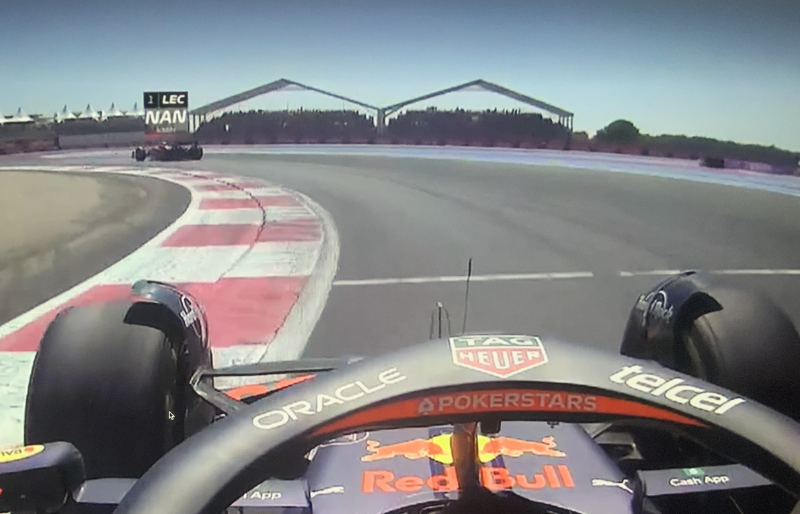
\includegraphics[width = 10cm]{../../Commun/Images/python-cours-nan}\\
    Charles Leclerc semble avoir un problème sur l'un de ses capteurs de vitesse
  \end{center}
  % \begin{exoUnique}
  %   \exo Quel est le nombre  $x$ qui est représenté en flottant par
  %   \begin{center}
  %   \begin{tabular}{|c||c|c|c|c|c|c|c|c|c|c|c||c|c|c|c|c|c|c|c|c|c|c|c|c|}
  %   \hline
  %   1&1&0&0&0&0&0&0&0&0&1&1&0&1&0&0&1&0&0&0&0&0&0&0&...\\
  %   \hline
  %   \end{tabular}
  %   \end{center}
  %   % \end{tabular}
  %   % \[\boxed{1}
  %   % \boxed{1}\boxed{0}\boxed{0}\boxed{0}\boxed{0}\boxed{0}\boxed{0}
  %   % \boxed{0}\boxed{0}\boxed{1}\boxed{1}%fin exposant
  %   % \boxed{0}\boxed{1}\boxed{0}\boxed{0}\boxed{1}
  %   % \boxed{0}\boxed{0}\boxed{0}\boxed{0}\boxed{0}\boxed{0}\boxed{0}\boxed{0}\boxed{0}\boxed{0}
  %   % \boxed{0}...\]
  %   la suite n'ayant ensuite que des $0$ pour avoir au total 64 bits~?
  %   \begin{sol}
  %   \begin{itemize}
  %   \item[$\bullet$] Le premier bit vaut $1$ donc c'est un nombre négatif.
  %   \item[$\bullet$] Les 11 bits suivants $\boxed{1}\boxed{0}\boxed{0}\boxed{0}\boxed{0}\boxed{0}\boxed{0}
  %   \boxed{0}\boxed{0}\boxed{1}\boxed{1}$ codent $e'$, l'exposant $e$ augmenté de $1023$. On a $e' = 2^{10}+0+0+0+0+0+0+0+0+2^1+2^0=1024+2+1=1027$. 
  %   Donc $e=e'-1023=4$.
  %   \item[$\bullet$] Les 52 bits restants sont $\boxed{0}\boxed{1}\boxed{0}\boxed{0}\boxed{1}$ puis que des $0$, cela code $m-1=\dfrac{0}{2}+\dfrac{1}{4}+\dfrac{0}{8}+\dfrac{0}{16}+\dfrac{1}{32}$.\\
  %   Donc $m=1+\dfrac{8+1}{32}=\dfrac{41}{32}$.
  %   \item[$\bullet$] Enfin, $x=-\dfrac{41}{32}\times 2^4=-\dfrac{41}{2}=-20,5$.
  %   \end{itemize}
  %   \end{sol}
  %   \end{exoUnique}

    
  

\subsection{Problèmes liés à l'arithmétique des nombres flottants}

\subsubsection{Overflow et underflow}
Le problème le plus simple à comprendre est celui du dépassement arithmétique (\emph{overflow} en anglais), qui
survient lorsqu'on dépasse le plus grand nombre représentable, qui est de l'ordre
de $10^{308}$ en double précision. Dans ce cas, le résultat est
$+\infty$ ou $-\infty$.

\begin{pythoncode}
In [1]: a = 2.0**1023

In [2]: a
Out[2]: 8.98846567431158e+307

In [3]: 2.0 * a
Out[3]: inf
\end{pythoncode}

\begin{sol}
Quelques explications pour les dernières lignes :
$$\sum_{k=0}^{53}\frac{1}{2^k}\times 2^{1023}=\p{2-\p{\frac{1}{2}}^{53}}\times 2^{1023}$$ Cette mantisse étant théoriquement égale à $2-\p{\frac{1}{2}}^{53}$, python la voit égale à $2$, donc ce nombre est $2^{1024}$, d'où "inf".\\
En revanche, 
$$\sum_{k=1}^{53}\frac{1}{2^k}=1-\p{\frac{1}{2}}^{53}=\p{2-\p{\frac{1}{2}}^{52}}\times 2^{-1}.$$ Donc sa mantisse est exacte, ce qui n'est plus le cas lorsqu'on ajoute $1$ comme le montre l'exemple précédent.
\end{sol}

\noindent
De même, pour les flottants strictement positifs, il peut y avoir dépassement par valeurs inférieures, ou \textit{underflow}. Dans
ce cas, le nombre renvoyé est 0 (plus précisément $0^+$ dans notre cas).

\begin{pythoncode}
In [4]: 2.0**(-1074)
Out[4]: 5e-324

In [5]: 2.0**(-1075)
Out[5]: 0.0
\end{pythoncode}
\noindent
Des études ont montré que même lors de calculs intermédiaires, de tels nombres
n'apparaissaient presque jamais. Ces problèmes peuvent donc essentiellement être ignorés.

\subsubsection{Inexactitude de la représentation, arrondis}

Les arrondis sont plus problématiques et sont liés au fait que les nombres
flottants n'ont qu'un nombre fini de chiffres significatifs. Deux types d'arrondis
entrent en jeu.\\

Le premier est dû au fait que les ordinateurs travaillent en base 2 alors qu'ils
échangent le plus souvent des informations avec l'utilisateur et le programmeur en base 10. Par exemple, lorsqu'on écrit
\begin{pythoncode}
In [1]: x = 0.1

In [2]: x
Out[2]: 0.1
\end{pythoncode}
on pourrait facilement être dupé et croire  que $0.1$ est représentable de
manière exacte en double précision. Or $0.1=1/10$ n'appartient à aucun des $\mathcal{F}_p$
puisque 10 n'est pas une puissance de 2. Il n'est donc pas représentable de manière exacte
par un nombre flottant, un peu comme $1/7=0.142857\underline{142857}$ n'est pas un nombre
décimal (le souligné signifie que le groupe de chiffres se répète à l'infini). Si l'on effectue un
développement de $1/10$ en base 2, on obtient $1.100\underline{1100} \times 2^{-4}$ (encore une fois, le groupe de chiffres se répète à l'infini).
Lorsque $0.1$ est entré dans le shell, Python va effectuer son développement en base
2. Comme ce développement est infini et qu'il travaille en double précision, il ne va garder que les 53 premiers bits
et arrondir $0.1$ à un nombre légèrement différent, avant de stocker ce nombre dans $x$. C'est un \emph{arrondi de conversion} de bases. Pour afficher
la valeur de $x$ à l'utilisateur, il va le reconvertir en base 10 et un autre arrondi de conversion
va faire qu'il affiche $0.1$. Mais il ne faut pas oublier que ce n'est pas $0.1$ qui est
stocké dans $x$.\\

Le second problème est plus fondamental~: les ensembles $\mathcal{F}_p$ ne sont
stables ni par addition, ni par soustraction, ni par multiplication; encore moins par
division. Par exemple
\[x\defeq (1+0/2+1/4)\times 2^1 \in\mathcal{F}_3 \quad\text{et}\quad
  y\defeq (1+0/2+0/4)\times 2^{-2}\in\mathcal{F}_3,\]
mais
\[x+y=(1+0/2+1/4+1/8)\times 2^1\not\in\mathcal{F}_3\]
car $x+y$ possède 4 chiffres significatifs. Pour chaque opération élémentaire (addition,
soustraction, multiplication, division) entre deux nombres flottants, le processeur se
trouve donc dans l'incapacité de
représenter le résultat exact par un nombre flottant~: il va devoir effectuer
un \emph{arrondi arithmétique}.
 Même si \verb_+_ et \verb_*_ restent commutatives,
ces arrondis leur font perdre leur associativité.
Plus le nombre d'opérations élémentaires
va être grand, plus ces arrondis vont nous éloigner du résultat attendu.
\vspace{2ex}
\begin{exoUnique}
\exo Observez les lignes suivantes et commentez.
\begin{pythoncode}
In [1]: 1.0 + 2.0**(-53) + (-1.0)
Out[1]: 0.0

In [2]: 1.0 + (-1.0) + 2.0**(-53)
Out[2]: 1.1102230246251565e-16
\end{pythoncode}
\begin{sol}
C'est dû au fait que l'ordinateur effectue les opérations dans l'ordre de lecture !
\begin{itemize}
\item[$\bullet$] Pour \texttt{1 + 2**(-54) - 1} :\\ L'ordinateur  commence par faire $1 + 2^{-54}$ :
signe $\epsilon = 1$, mantisse $m=1+2^{-54}$ et 
$e=0$ car c'est directement un nombre de $[1,2[$.
Problème :  $m$ vaut $1$ à $2^{-52}$ près, donc $m$ est stockée comme étant égale à $1$. \\Il est donc logique que lorsqu'on soustrait $1$, l'ordinateur réponde $0$ !!\\
\\

\item[$\bullet$] Pour \texttt{1 - 1 + 2**(-54) } :\\
Il fait d'abord $1-1$ qui vaut $0$ puis ajoute $2^{-54}$, qui lui est codé de manière exacte en machine : $\epsilon = 1$,  $m=1$ et $e = -54$. 
\end{itemize}
\end{sol} 
\end{exoUnique}
\vspace{2ex}
Ces phénomènes ne sont pas anodins et ne doivent pas être pris à la légère. Par exemple, si l'on veut tester l'égalité de deux flottants et qu'il existe une légère différence entre
eux due aux arrondis, on aura un résultat surprenant~!

\begin{pythoncode}
In [3]: 0.1 + 0.1 + 0.1 == 0.3
Out[3]: False

In [4]: import math

In [5]: math.sqrt(10)**2 == 10.0 
Out[5]: False
\end{pythoncode}

\noindent
On retiendra qu'il ne faut jamais faire de test d'égalité entre deux nombres
flottants. En pratique, on ne se posera pas la question de savoir si \verb!a == b!, mais
plutôt de savoir si \verb!abs(a - b) <= eps * abs(a)! où \verb!eps! est un nombre
\og petit \fg, à choisir selon notre application ($\epsilon\defeq\sqrt{u}\approx 10^{-8}$
est souvent un bon choix).\\

Nous avons vu pour le moment des calculs où les erreurs introduites par les arrondis
étaient négligeables devant les grandeurs manipulées. Mais ce n'est pas toujours le
cas. Supposons par exemple que l'on souhaite calculer
\[u_n\defeq\integ{0}{1}{x^n \e^x}{x}\]
pour tout $n\in\N$. Un encadrement élémentaire de l'intégrande nous montre que
\[\forall n\in\N\qsep 0\leq u_n\leq \integ{0}{1}{x^n \e}{x}=\frac{\e}{n+1}\]
ce qui prouve par le théorème des gendarmes que $u_n$ tend vers
0 lorsque $n$ tend vers $+\infty$. Si l'on veut calculer explicitement $u_n$, 
on remarque que $u_0=\e-1$ et une intégration par partie nous donne
\[\forall n\in\N\qsep u_{n+1}=\e-(n+1) u_{n}.\]
Le programme suivant permet donc de calculer $u_n$.
\begin{pythoncodeline}
import math

def integrale(n):
    """integrale(n: int) -> float"""
    u = math.exp(1.0) - 1.0
    for k in range(n):
        u = math.exp(1.0) - (k + 1) * u
    return u
\end{pythoncodeline}
\begin{pythoncode}
In [6]: [integrale(n) for n in [0, 5, 10, 20]]
Out[6]: [1.718281828459045, 0.395599547802016,
         0.22800151529345358, -129.26370813285942]
\end{pythoncode}
Les premières valeurs de $u_n$ calculées sont réalistes, mais $u_{20}$ est
totalement faux. Ce phénomène
était prévisible, car si $\alpha\in\R$ et $(v_n)$ est la suite définie par
\[v_0\defeq\alpha\qsep \text{et}\quad \forall n\in\N\qsep v_{n+1}\defeq \e-(n+1)v_n\]
alors, en définissant l'erreur $\epsilon_n\defeq v_n-u_n$, on obtient facilement $\epsilon_{n+1} = -(n+1)\epsilon_n$ et donc
\[\forall n\in\N\qsep \epsilon_n=(-1)^n n! \epsilon_0.\]
Si $\alpha$ est une valeur approchée de $\e - 1$ telle que $\abs{\epsilon_0} = \abs{\alpha - (\e - 1)} \propto 10^{-16}$, comme $20! \propto \times10^{18}$, on en déduit que
$\abs{v_{20}-u_{20}}\propto 100$. Donc si l'on effectue une erreur de calcul de l'ordre de
$10^{-16}$ pour $u_0$, même si les calculs suivants sont exacts, l'erreur absolue
obtenue pour le $20^e$ terme de la suite $(u_n)$ est de l'ordre de 100, ce qui
est beaucoup plus grand que l'ordre de grandeur de $u_{20}$ puisque $0\leq u_{20}\leq \e/21\approx 0.13$. Certains
algorithmes numériques comme celui-ci sont \emph{instables} et rendent les calculs avec
des nombres flottants inexploitables. D'autres sont \emph{stables} et peuvent donc
être utilisés avec des nombres flottants. L'étude de la stabilité des algorithmes
numériques dépasse le cadre du programme des classes préparatoires.
% Pour tout $n\in\N$, on pose

% \begin{questions}
% \question Montrez que pour tout $n\in\Ns$, $u_n=e-n u_{n-1}$.
% \question En d\'eduire une fonction calculant $u_n$.
% \question Testez cette fonction pour diff\'erentes valeurs de $n$. Expliquez ce qu'il se passe.

% Pire, les arrondis arithmétique peuvent s'accumuler très rapidement et renvoyer
% des résultats complétements abbérants.

% \begin{exos}

% \exo On considère le programme suivant qui nous donne le nombre de racines du
%   polynôme $P\defeq aX^2+bX+c$.
% \begin{pythoncode}
% def nb_solutions(a, b, c):
%     """nb_solutions(a: float, b: float, c: float) -> int"""
%     delta = b**2 - 4 * a * c
%     if delta == 0:
%         return 1
%     elif delta > 0:
%         return 2
%     else:
% 				return 0
% \end{pythoncode}
% Tester et commenter ce code avec les trinômes $X^2+1.4X+0.49$ et $X^2+0.2 X+0.01$. Expliquer
% ce qui se passe.
% \begin{sol}
% 	\begin{pythoncode}
% 	>>> nbsolutions(1, 1.4, 0.49)
% 	0
% 	>>> nbsolutions(1, 0.2, 0.01)
% 	2
% 	\end{pythoncode}
% \end{sol}
% \end{exos}

% D'autres erreurs d'arrondis peuvent survenir lors de calculs, notamment entre des nombres dont les ordres de grandeur sont très différents. Par exemple
% \begin{pythoncode}
% >>> 2.0**(60) + 1 - 2.0**(60)
% 0.0
% \end{pythoncode}

% \begin{sol}
% \emph{Explication} : 

% L'ordinateur commence par faire $2^{60}+1$. C'est $2^{60}\times (1+2^{-60})$, donc  $\epsilon=1$, l'exposant $e=60$ et la mantisse est $m=1+ 2^{-60}$. $m$ est donc stocké comme égal à $1$, donc dans l'ordinateur $2^{60}+1$ est stocké comme $2^{60}$. Il est donc logique que lorsqu'on soustrait $2^{60}$, l'ordinateur réponde $0$ !!
% \end{sol}


% \begin{exoUnique}
% \exo Observez les lignes de commande suivantes et commentez.
% \begin{pythoncode}
% >>> 1 + 2**(-54) - 1
% 0.0
% >>> 1 - 1 + 2**(-54)
% 5.551115123125783e-17
% \end{pythoncode}
% \begin{sol}
% C'est dû au fait que l'ordinateur effectue les opérations dans l'ordre de lecture !
% \begin{itemize}
% \item[$\bullet$] Pour \texttt{1 + 2**(-54) - 1} :\\ L'ordinateur  commence par faire $1 + 2^{-54}$ :
% signe $\epsilon = 1$, mantisse $m=1+2^{-54}$ et 
% $e=0$ car c'est directement un nombre de $[1,2[$.
% Problème :  $m$ vaut $1$ à $2^{-52}$ près, donc $m$ est stockée comme étant égale à $1$. \\Il est donc logique que lorsqu'on soustrait $1$, l'ordinateur réponde $0$ !!\\
% \\

% \item[$\bullet$] Pour \texttt{1 - 1 + 2**(-54) } :\\
% Il fait d'abord $1-1$ qui vaut $0$ puis ajoute $2^{-54}$, qui lui est codé de manière exacte en machine : $\epsilon = 1$,  $m=1$ et $e = -54$. 
% \end{itemize}
% \end{sol}
% \end{exoUnique}




% %\newpage
% \subsection{Le problème de la comparaison à $0$}
% Une des conséquences principales est qu'un test \texttt{a == 0} n'a pas de sens si \texttt{a} est un flottant, puisque celui-ci a pu souffrir d'erreurs d'arrondis. \\%Illustrons ce problème avec des équations du second degré.\\
%  Par exemple, le programme suivant renvoie le nombre de solutions réelles d'une équation du second degré donnée par ses coefficients $a,b,c$ : 

% Le programme utilisait le test \texttt{Delta == 0}, mais  la variable \texttt{Delta} est de type flottant et a subi une erreur d'arrondi. Alors que la valeur théorique de \texttt{Delta} est de 0 pour nos deux exemples, cela a donne un nombre proche de 0 mais négatif dans le premier cas, positif dans le second cas.

% Que suggérez-vous pour éviter ce problème ?

% \bigskip
% \bigskip
% \bigskip
% \bigskip
% \bigskip
% \bigskip

% \begin{sol}La parade classique est de remplacer le test  \texttt{Delta == 0} par  \texttt{abs(Delta)< epsilon} (où \texttt{abs} est la valeur absolue). On choisira \texttt{epsilon} proche de 0, en fonction de notre problème (en particulier en fonction de l'ordre de grandeur des données que l'on utilisera en pratique).\end{sol}

\subsubsection{Quelques catastrophes dues à une mauvaise utilisation des nombres flottants}

Il y a un nombre de catastrophes qui sont
attribuables à une mauvaise gestion de l'arithmétique des nombres flottants.
Dans le premier exemple, cela s'est payé en vies humaines.

\begin{itemize}
\item \emph{Missile Patriot} : En février 1991, pendant la guerre du Golfe, une batterie américaine de
missiles Patriot, à Dharan (Arabie Saoudite), a échoué dans l'interception d'un
missile Scud irakien. Le Scud a frappé un baraquement de l'armée américaine
et a tué 28 soldats. La commission d'enquête a conclu à un calcul incorrect du
temps de parcours du scud, dû à un problème d'arrondi. Les nombres étaient représentés
en virgule fixe sur 24 bits. Le temps était compté par
l'horloge interne du système en dixièmes de seconde. Malheureusement, 1/10 n'a pas
d'écriture finie dans le système binaire : 1/10 = 0.1 (dans le système décimal)
= 0.0001100110011001100110011... (dans le système binaire). L'ordinateur de
bord arrondissait 1/10 à 24 chiffres, d'où une petite erreur dans le décompte
du temps pour chaque dixième de seconde. Au moment de l'attaque, la batterie
de missile Patriot était allumée depuis environ 100 heures, ce qui a entrainé
une accumulation des erreurs d'arrondi de 0.34 s. Pendant ce temps, un missile
Scud parcourt environ 500 m, ce qui explique que le Patriot soit passé à côté de
sa cible. Ce qu'il aurait fallu faire c'est redémarrer régulièrement le système
de guidage du missile.
% \begin{center}
%   \includegraphics[width = 6cm]{../../Commun/Images/info-cours-memoire-patriot}\\
%   Un missile patriot.
% \end{center}
% \vspace{2ex}
\item \emph{Bourse de Vancouver} : Un autre exemple où les erreurs de calcul ont conduit à une erreur notable
est le cas de l'indice de la Bourse de Vancouver. En 1982, elle a créé un nouvel
indice avec une valeur nominale de 1000. Après chaque transaction boursière,
cet indice était recalculé et tronqué après le troisième chiffre décimal et, au bout
de 22 mois, la valeur obtenue était 524.881, alors que la valeur correcte était
1098.811. Cette différence s'explique par le fait que toutes les erreurs d'arrondi
étaient dans le même sens : l'opération de troncature diminuait à chaque fois la
valeur de l'indice.
\end{itemize}

\section{Caractères et chaines de caractères}

\subsection{Codes ASCII et Unicode}

Le code ASCII associe un caractère à chaque entier entre 0 et 127, ce qui
correspond à 7 bits non signés. Ces caractères peuvent être classés en
trois grandes catégories~:
\begin{itemize}
  \item\emph{Caractères alphanumériques :} les chiffres et les lettres minuscules
        et majuscules. Seules les lettres utilisées en anglais font partie
        du code ASCII, donc pas de «~é~», de «~ñ~», de «~\ss~»\dots
  \item\emph{Autres caractères imprimables :} les signes de ponctuation, quelques
        symboles ()\verb!+!, \verb!*!, \verb!}!, etc) et l'espace.
  \item\emph{Caractères non imprimables~:} la tabulation, les différents caractères
        correspondant à un retour à la ligne, le caractère nul, etc.
\end{itemize}


\begin{center}
  \begin{tabular}{|c||c|c|c|c|c|c|c|c|c|c|}
  \hline
  &0&1&2&3&4&5&6&7&8&9\\
  \hline
  \hline
  0&\cellcolor[gray]{0.9}&\cellcolor[gray]{0.9}&\cellcolor[gray]{0.9}&\cellcolor[gray]{0.9}&\cellcolor[gray]{0.9}&\cellcolor[gray]{0.9}&\cellcolor[gray]{0.9}&\cellcolor[gray]{0.9}&\cellcolor[gray]{0.9}&\cellcolor[gray]{0.9}\\
  \hline
  10&\cellcolor[gray]{0.9}&\cellcolor[gray]{0.9}&\cellcolor[gray]{0.9}&\cellcolor[gray]{0.9}&\cellcolor[gray]{0.9}&\cellcolor[gray]{0.9}&\cellcolor[gray]{0.9}&\cellcolor[gray]{0.9}&\cellcolor[gray]{0.9}&\cellcolor[gray]{0.9}\\
  \hline
  20&\cellcolor[gray]{0.9}&\cellcolor[gray]{0.9}&\cellcolor[gray]{0.9}&\cellcolor[gray]{0.9}&\cellcolor[gray]{0.9}&\cellcolor[gray]{0.9}&\cellcolor[gray]{0.9}&\cellcolor[gray]{0.9}&\cellcolor[gray]{0.9}&\cellcolor[gray]{0.9}\\
  \hline
  30&\cellcolor[gray]{0.9}&\cellcolor[gray]{0.9}&&!&"&\#&\$&\%&\&&'\\
  \hline
  40&(&)&*&+&,&-&.&/&0&1\\
  \hline
  50&2&3&4&5&6&7&8&9&:&;\\
  \hline
  60&<&=&>&?&@&A&B&C&D&E\\
  \hline
  70&F&G&H&I&J&K&L&M&N&O\\
  \hline
  80&P&Q&R&S&T&U&V&W&X&Y\\
  \hline
  90&Z&[&\textbackslash&]&\char`\^&\_&\`\ &a&b&c\\
  \hline
  100&d&e&f&g&h&i&j&k&l&m\\
  \hline
  110&n&o&p&q&r&s&t&u&v&w\\
  \hline
  120&x&y&z&\{&|&\}&\char`\~&\cellcolor[gray]{0.9}&&\\
  \hline
  \end{tabular}
  \end{center}
  

Comme les caractères étaient presque systématiquement codés sur 8 bits,
les codes 128 à 255 étaient «~libres~» : ils ont pendant très longtemps
été utilisés pour coder les caractères spécifiques aux différentes
langues (signes diacritiques, lettres supplémentaires, etc). Cependant
ces extensions posaient deux problèmes :
\begin{itemize}
  \item Elles n'étaient pas standardisées, puisqu'elles différaient d'une
        langue à l'autre et qu'il y avait même plusieurs extensions
        concurrentes pour une même langue. En pratique, jusqu'à la
        fin des années 2000, il y avait une chance sur deux que tous les
        caractères accentués contenus dans un mail soient remplacés par
        une bouillie infâme avant de parvenir au destinataire.
  \item Elles permettaient plus ou moins de gérer les langues européennes
        ou au moins les langues basées sur l'alphabet latin, mais étaient
        totalement inappropriées au chinois, au japonais, etc.
\end{itemize}
\vspace{2ex}

Le standard Unicode a été développé à partir de la fin des années 1980. À l'heure
actuelle, il définit des codes pour \nombre{144\ 697} caractères, ce qui
permet de gérer l'ensemble des langues, ainsi que de nombreux caractères
supplémentaires comme les Emojis, par exemple. Ce standard définit
trois représentations binaires UTF-8, UTF-16 et UTF-32, et il est assez
complexe : nous ne rentrerons pas dans les détails. Dans tous les cas,
les \emph{codepoints} (l'entier associé à un caractère) ne sont pas
modifiés pour les caractères appartenant au code ASCII.
On peut obtenir un caractère à partir de son code Unicode grâce à la fonction
\verb!chr!.

\begin{pythoncode}
In [1]: ord('A')
Out[1]: 65

In [2]: ord('é')
Out[2]: 233
\end{pythoncode}
  
  \noindent
  On peut obtenir un caractère à partir de son code \textsc{Unicode} grâce à la fonction
  \verb!chr!.
  C'est d'ailleurs le moyen le plus simple d'obtenir des caractères non
  disponibles sur votre clavier.
  
% \begin{pythoncode}
% In [13]: "I " + chr(9829) + " les Lazos."
% Out[13]: 'I les Lazos.'
% \end{pythoncode}
\begin{lstlisting}[language=python, escapeinside=||]
In [3]: "I " + chr(9829) + " les Lazos."
Out[3]: 'I |
\includegraphics[width=0.25cm]{../../Commun/Images/python-cours-unicode-heart.png}| les Lazos.'
\end{lstlisting}

\subsection{Lecture et écriture dans un fichier}

Python permet d'ouvrir des fichiers texte en lecture ou en écriture. Pour Python, un
fichier n'est qu'une séquence de caractères. Une fois que le fichier aura été ouvert
par le programme, celui-ci maintiendra un marqueur fictif à la position courante qui
nous indique où sera lue ou écrit la prochaine séquence. Un fichier est ouvert avec la
fonction \verb!open!~:

\begin{pythoncode}
f = open("/Users/fayard/Desktop/fichier.txt", 'r')
\end{pythoncode}
\noindent
Le premier argument est une chaine de caractères contenant le chemin complet du fichier.
Le second argument est le mode d'ouverture du fichier~: \verb_'r'_ (pour read)
pour une ouverture en lecture seule, \verb_'w'_ (pour write)
pour une ouverture avec les droits d'écriture et enfin \verb_'a'_ (pour append)
pour une ouverture avec les droits d'écriture et la position du marqueur en fin
de fichier. Une fois que le travail dans le fichier sera fini, il faudra prendre soin
de bien fermer le fichier avec la commande
\begin{pythoncode}
f.close()
\end{pythoncode}

\medskip
Une fois ouvert, la fonction \verb!read! permet de lire le fichier en entier et le renvoie sous la forme
d'une chaine de caractères~:
\begin{pythoncode}
texte = f.read()
\end{pythoncode}
Dans la même famille, la fonction \verb!readlines()! permet de lire le fichier en entier,
mais renvoie non pas une seule chaine de caractères, mais une liste de chaines
de caractères, chaque chaine correspondant à une ligne du fichier. Attention, cette
ligne se terminera par le caractère de retour à la ligne.
\begin{pythoncode}
lignes = f.readlines()
\end{pythoncode}
Mais en général, on lira et on traitera le fichier ligne par ligne avec le fonction
\verb!readline()! qui lit une ligne et la renvoie en tant que chaine de caractères.
Bien entendu, cette chaine finira aussi par un caractère de retour à la ligne. Après
cet appel, le curseur sera positionné au début de la ligne suivante.
\begin{pythoncode}
ligne = f.readline()
\end{pythoncode}
On saura qu'on est à la fin du fichier lorsque cette méthode nous renverra une chaine
de caractères vide.\\

Mais la méthode sans doute la plus utilisée pour parcourir un fichier
en lecture est de remarquer que le descripteur du fichier \verb!f! est un itérable.
La boucle
\begin{pythoncode}
for ligne in f:
\end{pythoncode}
va donc permettre d'effectuer une boucle sur toutes les lignes du fichier. Cette boucle
est équivalente à
\begin{center}
  \verb!for ligne in f.readlines():!
\end{center}
mais a l'avantage de faire lire le fichier à notre programme ligne après ligne alors que
l'utilisation de \verb!readlines()! va charger le fichier en mémoire en entier avant même
de traiter la première ligne.\\

Il est courant de lire des fichiers textes contenant des données organisées, comme
par exemple un fichier \textsc{Csv} (Comma Separated Values) qui est le format le
plus simple pour enregistrer les données d'un tableur. Le fichier décrit dans un fichier
texte chaque ligne du document, où chaque colonne est séparée par une virgule. Si par
exemple, vous souhaitez avoir une liste des élèves de la classe avec leur âge, le fichier
\textsc{Csv} correspondant sera simplement
\begin{pythoncode}
Linus,Torvalds,53
Donald,Knuth,85
Master,Yoda,900
\end{pythoncode}
Afin de séparer proprement ce type de ligne, on utilisera la fonction \verb!split!.
Par exemple, si \verb!ligne! est égal à \verb!"Linus,Torvalds,53"!, la commande
\verb!data = ligne.split(',')! stockera dans la variable \verb!data! la liste
\begin{center}
\verb!["Linus", "Torvalds", "53"]!.
\end{center}

Si le fichier est ouvert en écriture, on peut écrire dedans à l'aide de la méthode
\verb!write!.
\begin{pythoncode}
f.write("Ma jolie histoire.")
\end{pythoncode}

\medskip
Le programme spécifie que la documentation de ces fonctions doit vous être rappellée
mais il est important de savoir les utiliser proprement une fois ce rappel fait.


% \section{La mémoire}
% \subsection{Des 0 et des 1}

% Un ordinateur possède une mémoire vive, appelée {\sc RAM} pour \og Random Access Memory\fg. C'est cette mémoire qui matérialise l'état du système dont nous parlions dans le chapitre sur les variables. En pratique, ces \og barrettes mémoire \fg contiennent des milliards de condensateurs qui peuvent chacun être soit chargés, soit déchargés.

% % \begin{center}
% % \includegraphics[width=0.6\textwidth]{ram.jpg}
% % \end{center}

% Si on note $n$ le nombres de condensateurs présents dans la RAM de l'ordinateur, en indexant ces condensateurs de $0$ à $n-1$, on peut représenter l'état de la mémoire par un tableau de 0 et de 1. L'état 0 signifie que le condensateur est déchargé et l'état 1 signifie qu'il est chargé.

% \begin{center}
% \begin{tabular}{|l||c|c|c|c|c|c|c|c|c|c|c|c|}
% \hline
% condensateur & 0 & 1 & 2 & 3 & 4 & 5 & 6 & 7 & 8 & 9 & $\ldots$ & $n-1$ \\
% \hline
% état & 0 & 1 & 0 & 0 & 1 & 0 & 1 & 1 & 0 & 0 & $\ldots$ & 1\\
% \hline
% \end{tabular}
% \end{center}


% Pour enregistrer des données, un ordinateur possède un très grand nombre de \og bits \fg qui ne peuvent être que dans deux états~: 0 ou 1. En pratique, ce sont des condensateurs qui sont soit chargés, soit déchargés. Un bit suffit pour stocker un booléen. On prend la convention qui consiste à dire que si le bit est dans l'état 0, le booléen est faux et que si le bit est dans l'état 1, le booléen est vrai.\\

% Supposons maintenant que l'on souhaite stocker la direction de déplacement d'un joueur sur une carte et que seulement 4 directions sont possibles~: nord, sud, est, ouest. Pour cela, il nous suffit d'avoir 2 bits. On peut dire que par convention \verb_11_ représente le nord, \verb_00_ représente le sud, \verb_01_ représente l'est et \verb_10_ représente l'ouest.\\

% On comprend alors que 3 bits suffisent pour représenter 8 valeurs et plus généralement $n$ bits suffisent pour représenter $2^n$ valeurs. En particulier, avec 8 bits, vous pouvez représenter 256 valeurs. Un octet est formé de 8 bits. C'est la plus petite quantité de mémoire avec laquelle les ordinateurs travaillent. Un octet permet donc de stocker un nombre entre 0 et 255 inclus. En se mettant d'accord sur une correspondance entre les nombres et les caractères les plus élémentaires, on peut donc stocker un caractère sur un octet. La table de correspondance la plus utilisée est la table {\sc ASCII}. Un octet, c'est aussi
% généralement la mémoire demandée pour stocker la luminosité d'un pixel d'une image en noir et blanc. L'oeil peut difficilement discerner plus de 256 niveaux de gris et un ordinateur stocke donc le niveau de gris d'un pixel avec un nombre entre 0 et 255. L'octet est ainsi devenu l'unité de base pour décrire la quantité de mémoire. En anglais, un octet se dit \og byte\fg qu'il ne faut surtout pas confondre avec le \og bit\fg.\\

% La bible contient a peu pr\`es $4$ millions de caractères. Il faut donc le même nombre d'octets pour la stocker. Comme en physique avec le mètre et le kilomètre, on aimerait avoir une unité pour spécifier 1000 octets. Seulement, il se trouve que les puissances de 2 sont très utiles en informatique et que $2^{10}=1024$. Certaines personnes ont décidé de choisir qu'un kilooctet représente 1000 octets. D'autres ont décidé qu'un kilooctet représente 1024 octets. Certains organismes ont tranché et décidé qu'un kilooctet devait faire 1000 octets et que 1024 octets s'appeleraient un kibioctet. Autant vous dire que ces organisations sont autant écoutées que l'Académie Française quand elle demande d'écrire un {\sc cd-rom}, Cédérom. Après tout, la différence n'est que de 2\%, mais nous allons voir que les choses se gâtent quand on passe au mégaoctet. Pour certaines personnes, le mégaoctet représente 1024 ko (celui qui représente 1024 octets), soit $2^{20}$ octets. Pour d'autres, un mégaoctet, c'est simplement 1000 ko (celui qui représente 1000 octets) soit un million d'octets. La différence est maintenant d'à peu près 5\%. Quand on passe au gigaoctet, qui représente selon les personnes $2^{30}$ octets et selon les autres un milliard d'octets, la différence est de 7\%. Au téraoctet, la différence est de 10\%. Je vous laisse imaginer quel choix ont fait les vendeurs de disques durs. Dans ce cours, nous ne calculerons que des ordres de grandeur et la différence ne sera pas importante. On retiendra que la bible encodée en {\sc ASCII} occupe \`a peu près 4~Mo de mémoire. C'est à peu près la taille nécessaire pour stocker une chanson en {\sc MP3} dans une qualité standard. Si vous regardez un film sous \textsc{Netflix} en qualité haute définition, il faudra compter 1~Go. Le même film tel qu'il est diffusé dans un cinéma sera très peu compressé et utilisera \`a peu près 1~To. Pour information, un ordinateur portable actuel a souvent une {\sc RAM} de quelques Go (disons entre 2~Go et 32~Go) et un disque dur entre 256~Go et 8~To.\\

% On retiendra qu'avec suffisamment de 0 et de 1, on peut stocker \`a peu près n'importe quelle information. Il suffit juste de construire une correspondance entre les suites de 0 et de 1 et ces informations. Dans ce chapitre, nous allons décrire cette correspondance pour les entiers.

% \begin{exercicepython}{}
% Combien de bits sont-ils nécessaires pour repr\'esenter tous les \'el\`eves de la classe~?
% %\question On a 13 pièces d'or. Elles pèsent toutes 10~gr sauf une qui pèse 11~gr. On souhaite découvrir quelle est cette pièce à l'aide d'une balance à deux plateaux. Montrer que l'on peut déterminer la pièce plus lourde en 3 pesées. 
% \end{exercicepython}


%END_BOOK

\end{document}